%!TEX root=masterproef.tex

\section{Draadloze sensornetwerken}
\label{section:landscape}

``\emph{Waarom is het belangrijk om beveiliging van draadloze sensornetwerken
te bestuderen? Dit is toch al uitvoerig gedaan in andere vormen van
netwerken?}'' Op het eerste zicht is dit een zeer valabele vraag. Reeds sinds
de late jaren '80 kennen we concepten als \emph{firewalls} en virussen en
wormen. Meer dan 30 jaar reeds wordt er onderzoek gedaan naar
computerbeveiliging en solide oplossing zijn bedacht, uitgewerkt en
ge\"implementeerd. Wat houdt ons tegen om deze toe te passen op draadloze
sensornetwerken?

\subsection{Eigenschappen}

Ondanks het feit dat men knopen kan beschouwen als kleine computers en de
verbindingen die tussen hen tot stand komen een netwerk worden genoemd, eindigt
daar de vergelijking met andere bestaande technologie\"en volledig. Draadloze
sensoren en hun netwerken zijn een wereld op zich met zeer typerende
eigenschappen en eigen regels, mogelijkheden en beperkingen.

Een draadloze sensor is inderdaad een kleine computer, maar de nadruk ligt hier
op \emph{kleine}. De rekenkracht van een knoop is slechts een fractie van deze
van een hedendaagse computer en ligt in de tientallen megahertz (MHz), waar
hedendaagse systemen spreken in termen van gigahertz (GHz). De reden is
evident: draadloze sensornetwerken zijn volledig draadloos en worden ingezet in
de meest uiteenlopende, maar typisch afgelegen situaties. Ze zijn daarom
gedurende lange tijd afhankelijk van een zelfde batterijvoeding, en die moet
dan ook optimaal benut worden.

Ook het netwerk dat ze vormen vertoont typische eigenschappen die sterk
verschillen van de meer klassieke computernetwerken. Zo identificeert
\cite{blilat2012wireless} zes unieke eigenschappen van draadloze
sensornetwerken die leiden tot specifieke uitdagingen en opportuniteiten:

\begin{enumerate}

\item{De routering van de meeste draadloze sensornetwerken is
\emph{gestructureerd als een boom}. De concepten co\"ordinator (of
basisstation), router en eindknoop werden eerder, samen met hun structuur,
ge\"identificeerd in sectie \ref{subsection:topologie}.}

\item{De gegevens die door een knoop in het netwerk worden verzameld worden
typisch niet op zich beschouwd, maar \emph{geaggregeerd} met de metingen van
andere knopen. Dit wordt enerzijds gedaan om te compenseren voor effectieve
aberraties in de metingen zelf, maar ook om de onzekerheid van de
beschikbaarheid van de knopen te ondervangen.}

\item{Knopen zijn typisch de goedkope onderdelen van het netwerk en ze staan
slechts ten dienst van het eigenlijke doel van het netwerk, het verzamelen van
gegevens. Om die reden zijn ze eenvoudig vervangbaar en wordt dit als een
inherente eigenschap gezien. Het netwerk \emph{tolereert storingen} ten gevolge
van het wegvallen van knopen en vangt ze op door redundantie en aggregatie.}

\item{Om er voor te zorgen dat het netwerk zo min mogelijk belast wordt met het
verzenden van gegevens, worden meetgegevens zo dicht mogelijk bij de
oorspronkelijke knoop \emph{gefilterd en verwerkt}.}

\item{Een draadloos sensornetwerk bestaat uit knopen en niets anders. Elke
knoop is tegelijkertijd een \emph{sensor en router}, wat resulteert in een
optimalisatie van het netwerkverkeer.}

\item{De werking van een knoop kent een typisch \emph{gefaseerd zendpatroon}:
het verzamelen van meetgegevens, het ontvangen van gegevens van andere knopen en
het doorsturen van geaggregeerde gegevens naar hoger liggende knopen. Hierdoor
kan elke knoop zijn zender gedurende bepaalde periodes volledig afzetten,
natuurlijk om energie te besparen.}

\end{enumerate}

Dit beeld vinden we ook terug bij \cite{aschenbruck2012security} die de
situatie van draadloze sensornetwerken samenvat in drie zeer typische en
problematisch bronnen van beveiligingsproblemen: de beperkingen qua middelen en
dan vooral de energievoorziening, de fysieke toegankelijkheid die leidt tot de
mogelijkheid van het veroveren van knopen en de verwerking van gegevens die
reeds binnen het netwerk gebeurt, waardoor het bv. onmogelijkheid om encryptie
toe te passen tussen zender en ontvanger, waardoor tussenliggende verwerking
uitgesloten wordt.

\subsection{Inbraakdetectie}

Maar ook het probleemgebied waarin draadloze sensornetwerken in deze thesis
vertoeven, maakt het op nog meer vlakken verschillend van een klassieke
computernetwerk.

In \cite{zhang2000intrusion} wordt een zeer algemene, maar zeer correcte
definitie gegeven van inbraak detectie.

\begin{quote}
\emph{Intrusion detection ... involves capturing audit data and reasoning about
the evidence in the data to determine whether the system is under attack.}
\end{quote}

Inbraakbeveiliging omvat twee essenti\"ele activiteiten: het vastleggen van
auditgegevens en het redeneren over deze gegevens. In het geval van draadloze
sensornetwerken moeten we het aspect \emph{systeem} op twee manieren
interpreteren: enerzijds als een knoop en anderzijds als het hele netwerk op
zich. Dit onderscheid bestaat ook in meer klassieke computernetwerken in de
vorm van \emph{systeem} en \emph{netwerk} inbraakdetectie.

In de context van draadloze sensornetwerken zal dit onderscheid zich echter
veel meer uitgesproken profileren omdat het netwerk hier geen centraal medium
is. Daar waar het netwerk in een klassieke opstelling typisch vanuit \'e\'en
systeem kon gecontroleerd worden door het afleiden van alle netwerkverkeer naar
\'e\'en enkele detectiemodule, is dit in het geval van een DSN niet langer
mogelijk. Het draadloze aspect maakt dat er geen controleerbare toegangswegen
meer zijn naar elke knoop en dat dus elke knoop letterlijk op zichzelf
aangewezen is.

Samen met het wegvallen van een centrale inbraakdetetie, valt ook de centrale
bescherming op netwerk niveau weg. Binnen een DSN is het ook niet mogelijk om
te genieten van de bescherming van een \emph{firewall}. Er is niet langer een
alles omarmende bescherming, niet op logisch of netwerk vlak, maar ook op
fysisch vlak. Aangezien draadloze sensornetwerken typisch open en bloot in de
buitenwereld ge\"installeerd worden, en dit voor langere periodes zonder
aanwezigheid van een eigenaar, kunnen ze ook fysiek benaderd worden door ieder
dat dat wil. Zelfs de elementaire zekerheid van een fysieke bescherming bv. in
een datacenter, komt bij draadloze sensornetwerken volledig te vervallen.

Zeer terecht stelt \cite{perrig2004security} daarom ook dat de eerste zorg
omtrent de beveiliging van draadloze sensor netwerken een veilige manier om de
groep van sensoren te beheren is. De manier waarop nieuwe knopen in het netwerk
worden opgenomen en de beveiliging van de onderlinge communicatie is van
primordiaal belang. Voorkomen is beter dan genezen.

Maar we moeten ook realistisch zijn. Geen door mensenhanden gemaakt systeem is
feilloos en nagenoeg elk ge\"informatiseerd system zal met de nodige inzet en
moeite veroverd kunnen worden. Op dat ogenblik is het belangrijk dat er een
tweede verdedigingslinie is: inbraakdetectie. In het geval van DSN is dit dus
misschien nog meer prangend, omdat er niet langer een fysieke bescherming is,
noch een centrale netwerkbescherming in de vorm van bv. een \emph{firewall}.

\subsection{De tegenstander en zijn aanvallen}

Tijd om kennis te maken met onze tegenstander. Wat is zijn doel? Welke middelen
heeft hij ter beschikking? Hoe kunnen we zijn aanvallen identificeren?

Identificatie van aanvallen wordt door \cite{zhang2000intrusion} gecatalogeerd
als \emph{misbruik} of \emph{anomalie}. Misbruik kan typisch gedetecteerd
worden aan de hand van patronen, terwijl voor het detecteren van anamolie\"en
er een patroon moet opgesteld worden en aberraties van dat patroon opgemerkt
moeten worden. Vooral dit laatste is typisch een delicaat aspect. Zo is het
onderscheid tussen een knoop die verplaatst werd en tijdelijk verkeerde routing
informatie verspreid en een knoop die veroverd werd en kwaadwillig foutieve
informatie uitstuurt, niet eenvoudig te maken.

\cite{aschenbruck2012security} identificeert vier fundamentele doelen die
nagestreefd worden door een aanvaller: (1) het manipuleren van gegevens, (2)
het afluisteren van communicatie, (3) het tegenhouden van gegevens en (4)
toegang verkrijgen tot het netwerk. Dezelfde doelen vinden we ook bv. terug bij
\cite{blilat2012wireless}, zij het in een andere opdeling: het afluisteren van
communicatie, het analyseren, verstoren en kapen van netwerkverkeer en fysieke
aanvallen.

Aanvallen kunnen volgens \cite{dargie2010fundamentals} ingedeeld worden in vijf
klassen: aanvallen die het netwerk weerhouden om zijn diensten te realiseren
(\emph{Denial-of-Service} or \emph{DoS}), aanvallen op het niveau van de
routing binnen het netwerk, aanvallen gericht op de transport algoritmes binnen
het netwerk, aanvallen op het aggregerende karakter van het netwerk en
aanvallen gericht op de privacy van de deelnemers in de werking van het netwerk.

\cite{aschenbruck2012security} ervaart DoS eerder als een doel en deelt de
aanvallen vervolgens op in vier licht verschillende categorie\"en die correcter
aansluiten bij een draadloos sensornetwerk: het fysieke niveau waar een
aanvaller gebruik maakt van middelen om het alomtegenwoordig draadloos netwerk
te benaderen, het niveau waarop het fysieke niveau benaderd wordt door de
knopen, de zgn. \emph{Medium-Access layer} of \emph{MAC} laag, het niveau van
de routering en het niveau van de knoop als een functionele eenheid. Het is
duidelijk dat er feitelijk een grote tweeledigheid wordt gecre\"eerd tussen
enerzijds het draadloze netwerk en anderzijds de knoop op zich. Op elk van deze
niveaus identificeert men vervolgens typerende aanvallen. Voor elk type van
aanval wordt tevens een mogelijke antwoord gedefinieerd.

Figuur \ref{fig:wsn-threat-analysis} geeft een schematisch overzicht van de
vier fundamentele doelen, de vier categorie\"en en de mogelijke antwoorden.

\begin{figure}[ht]
  \centering
  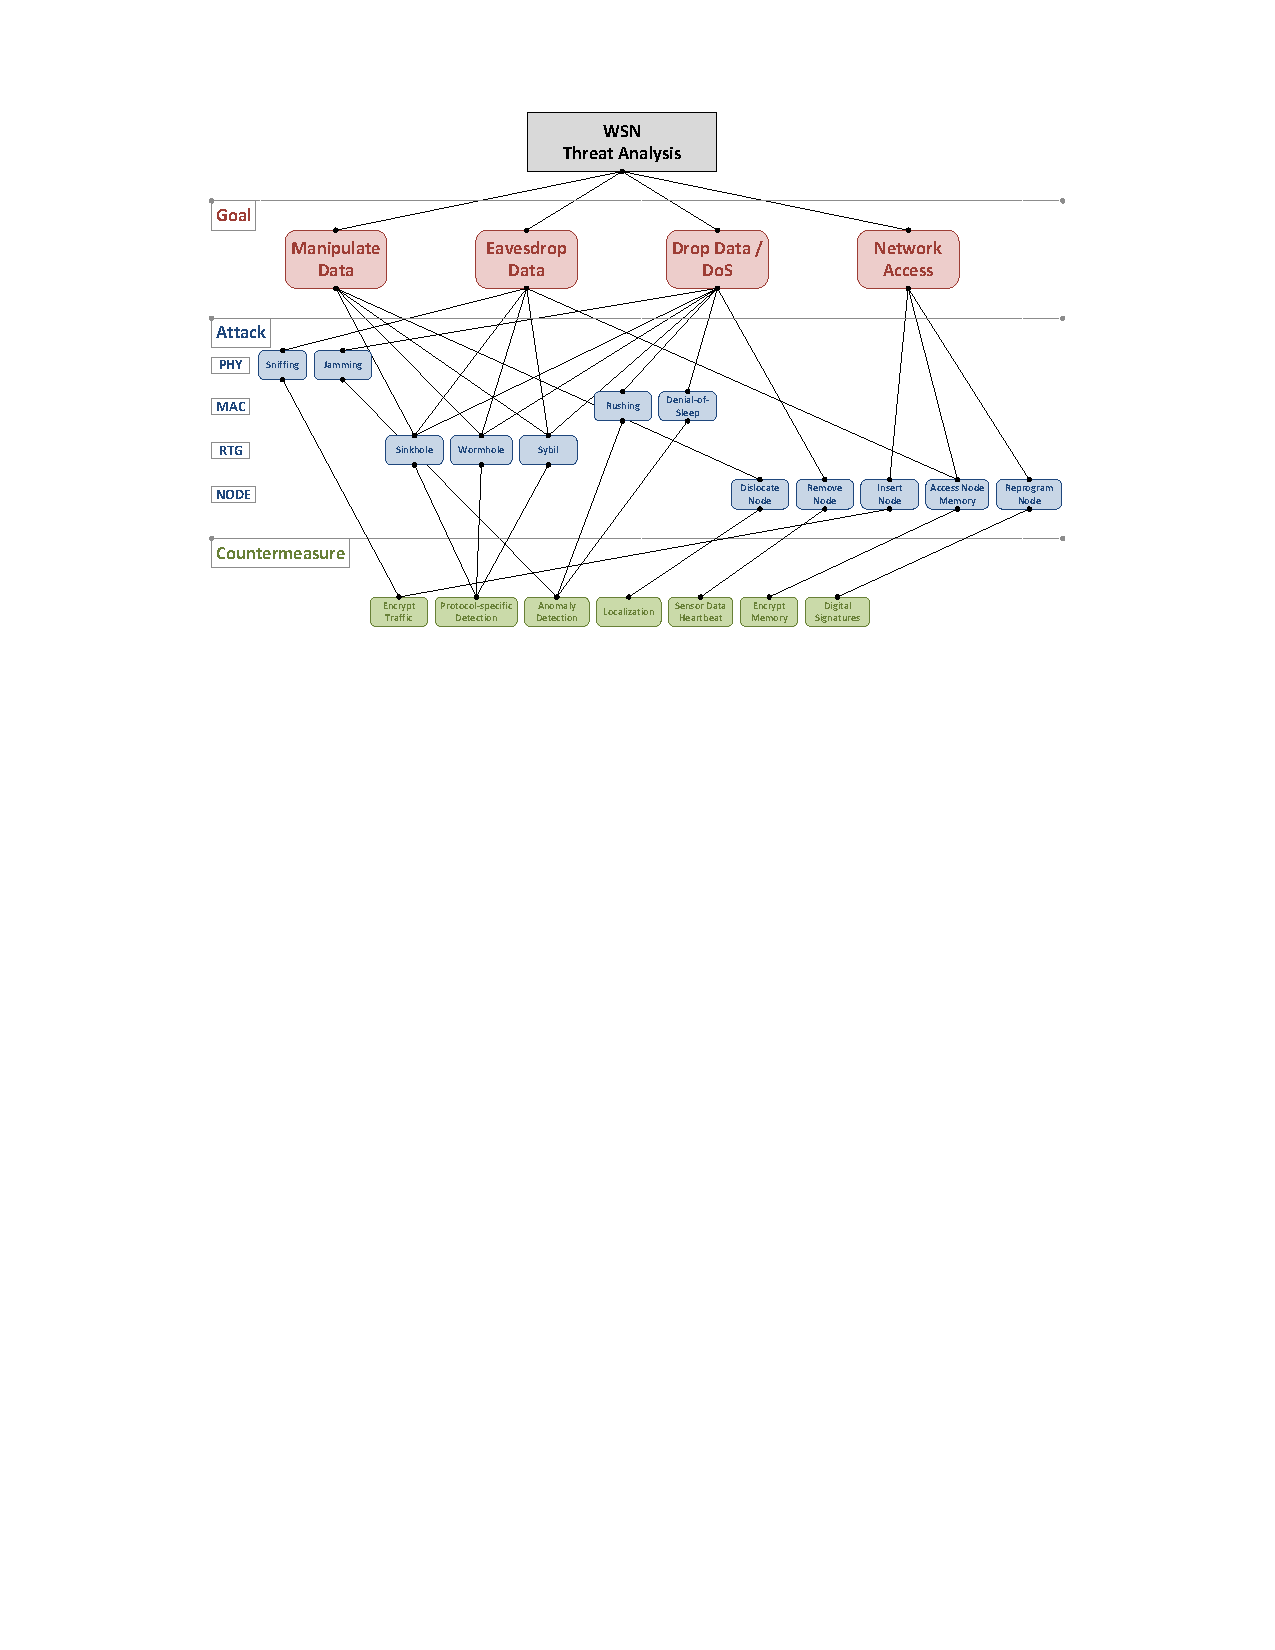
\includegraphics[width=0.9\linewidth]{resources/wsn-threat-analysis.pdf}
  \caption{Analyse van de bedreiging van een DSN.}
  \label{fig:wsn-threat-analysis}
\end{figure}

\subsubsection*{Fysieke laag}

De fysieke laag betreft het niveau van de effectieve radiogolven, de
communicatie zoals ze zich letterlijk door de lucht voortbeweegt. De naam is in
dit geval dus tegenstrijdig, aangezien er feitelijk totaal geen fysiek contact
met het DSN of de knopen gerealiseerd wordt.

Twee belangrijke types van aanvallen vinden hier plaats: \emph{snuffelen} of
\emph{afluisteren} (Engels: \emph{sniffing}) en \emph{storen} (Engels:
\emph{jamming}).

Aangezien communicatie als radiogolven van de ene node naar de andere node
plaatsvindt, kan in essentie iedereen met een radio-ontvanger deze golven
opvangen en omzetten in het dataverkeer dat aan de oorsprong ligt.

Een mogelijk antwoord op \emph{afluisteren} is het versleutelen van de
communicatie door middel van cryptografie. Hierdoor \emph{kan} men het de
aanvaller inderdaad moeilijker maken. Indien hij niet beschikt over de nodige
sleutels om de encryptie ongedaan te maken, kan hij echter nog steeds nuttige
informatie halen uit de hoeveelheid en types van pakketten die via het netwerk
verstuurd worden.

Aangezien het echter bijna steeds mogelijk is om het geheugen van een knoop te
analyseren zonder dat deze hiervan enige weet heeft, is een aanvaller in
theorie in staat om de nodige sleutels uit een gewone sensorknoop uit te halen
en deze te gebruiken om het netwerkverkeer te ontcijferen en ook de inhoud
volledig te kunnen bekijken en analyseren.

\emph{Afluisteren} is een passieve aanval. Op zich worden er geen acties
ondernomen die wijzigingen aanbrengen in het netwerk, die op hun beurt kunnen
gedetecteerd worden. Bij het \emph{storen} van het netwerk is dit wel het geval.

Door gebruik te maken van een sterke radio-zender, kan een aanvaller de
radiogolven van het netwerk zo verstoren dat valide communicatie niet langer op
een goede manier realiseerbaar is.

Om het \emph{storen} van het netwerk te detecteren kan me gebruik maken van
anomaliedetectie. Verhoging van parameters zoals de \emph{carrier sense time}
(CST), de tijd nodig om toegang tot het netwerk te krijgen, kunnen een
aanduiding zijn dat het netwerk onnodig zwaar belast wordt en kunnen wijzen op
het \emph{storen} van het netwerk.

\subsubsection*{MAC laag}

Een draadloos netwerk is een gedeeld medium. Een draadloze radio kan slechts
\'e\'en signaal tegelijkertijd verwerken. Er kunnen dus nooit twee radio's op
het zelfde moment gegevens versturen. Om dit mogelijk te maken is er een niveau
nodig waar de verschillende radio's met elkaar afstemmen wanneer wie aan de
beurt is. Dat is de \emph{medium access layer} of MAC laag en gebeurt typisch
doordat alle knopen onderling dezelfde regels hanteren zodat er een eerlijke
verdeling ontstaat van het gebruik van het medium.

Dit samenwerkingsverbond kan echter natuurlijk geschonden worden en dit leidt
tot aanvallen zoals \emph{overrompelen} (Engels: \emph{rushing}) of het
\emph{ontzeggen van slaap} (Engels: \emph{denial of sleep}).

Indien een aanvaller zich niet houdt aan de regels van de MAC laag, en deze
zijn eigen pakketten sneller verstuurd dan de gewone knopen, zal dit de werking
van het MAC-niveau protocol verstoren, zullen de gewone knopen wachten met het
verzenden van hun pakketten en wordt de werking van het netwerk lam gelegd.

Opnieuw zal anomaliedetectie nodig zijn om deze situatie te detecteren,
gelijkaardig zoals bij het \emph{storen} van het netwerk.

De meeste energie van een knoop gaat op aan de draadloze communicatie. Het
MAC-niveau protocol bepaalt in grote mate hoeveel ruimte een knoop heeft om
zijn draadloze radio in slaapstand te plaatsen om het energieverbruik te
beperken.

Door eigenschappen van het MAC-niveau protocol te misbruiken kan een aanvaller
een zich correct gedragende knoop verplichten om zijn radio aan te laten staan
en hem zo \emph{ontzeggen van slaap}. Dit leidt natuurlijk tot het versneld
leeglopen van zijn batterij en uiteindelijk tot het beperken van de werking van
het netwerk van enkele maanden tot zelfs slechts enkele dagen.

Opnieuw kan aan de hand van anomaliedetectie abberaties in het energieverbruik
gedetecteerd worden en kan het standaard gedrag aangepast worden.

Gerelateerd aan deze aanvallen identificeren \cite{dargie2010fundamentals} en
\cite{djenouri2005survey} ook nog \emph{overspoelen} (Engels: \emph{flooding}).
Dit kan beschouwd worden als een specifieke variant van \emph{overrompelen},
waarbij de aanvaller herhaaldelijk communicatie initieert maar niet verderzet.
Hierdoor zal de knoop die aangevallen wordt geen mogelijkheden meer hebben om
andere, legitieme communicaties te ontvangen.

\subsubsection*{Routering laag}

Een niveau van abstractie hoger bevindt zich de routering laag. Hier wordt
bepaald naar welke knoop een bepaald bericht wordt verzonden om uiteindelijk
bij de juiste bestemmeling terecht te komen. Aangezien dit niveau bepaalt hoe
het normale communicatieverkeer verloopt, is dit niveau een uitermate
interessant gegeven voor aanvallers.

\'E\'en van de belangrijkste aspecten van een aanval op een DSN is het vergaren
van zoveel mogelijk informatie. Dit kan een doel op zich zijn, maar kan ook
nodig zijn om de eigenlijke aanval te ondersteunen. Zo zien we dat aanvallen op
dit niveau typisch bedoeld zijn om communicatie te af te luisteren, te
manipuleren of zelfs te onderdrukken. Zo onderscheiden we de \emph{Sinkhole},
\emph{Wormhole} en \emph{Sybil} aanvallen.

Bij een \emph{Sinkhole} aanval tracht de aanvaller zoveel mogelijk van het
netwerkverkeer naar zich toe te lokken \cite{krontiris2008launching}. Zo is hij
in staat om te doen wat hij wilt met dat verkeer: hij kan het analyseren,
aanpassen of zelfs gewoon niet doorsturen. Dit laatste wordt ook wel
\emph{selectief doorsturen} (Engeld: \emph{selective forwarding}) genoemd. De
aanvaller kan zijn veroverde knoop \emph{aantrekkelijk} maken voor andere
knopen op het niveau van routering. Door valselijk kortere toegangspaden naar
andere knopen aan te bieden, zullen knopen geneigd zijn om berichten langs de
\emph{Sinkhole} te verzenden.

\emph{Sinkhole} aanvallen zijn vrij moeilijk te detecteren. De reden is
evident, indien er een makkelijke manier was om zelf een korter pad te bepalen,
zou de informatie niet nodig zijn en zou de aanval zelfs niet eens bestaan. Het
is dus nagenoeg onmogelijk om valide routering informatie van valse te
onderscheiden.

Bij een \emph{Workhole} aanval zal de aanvaller twee punten in het netwerk met
elkaar verbinden door middel van een zeer snelle verbinding. Op die manier zijn
de twee punten vanuit het oogpunt van routering protocollen dicht bij elkaar en
zal er gebruik gemaakt worden van deze ``kortere'' weg. Net omdat deze
constructie in essentie niets verkeerd doet, is het opnieuw een aanval die zeer
moeilijk te detecteren valt.

Net zoals bij de \emph{Sinkhole} aanval, beschikt de aanvaller opnieuw over
grote hoeveelheden gegevens, waarmee hij opnieuw kan doen wat hij wil.

Een \emph{Sybil} aanval ontstaat wanneer \'e\'en enkele knoop meerdere
identiteiten opneemt en zo met \'e\'en knoop het verkeer van meerdere knopen
kan verwerken. Opnieuw is de aanvaller heer en meester over meer communicatie
dan normaal en kan deze controleren naar believen.

\subsubsection*{De knoop}

In tegenstelling tot hun grotere broertjes zijn sensorknopen fysiek te
benaderen. Terwijl onze computer veilig in ons huis staat of zich zelfs in een
datacenter bevindt, ligt de sensorknoop letterlijk voor het rapen. Zo ontstaat
er een rijkdom aan mogelijkheden voor een aanvaller om een knoop fysiek te
benaderen en kan hij een knoop \emph{verplaatsen}, \emph{verwijderen} en
\emph{toevoegen}. Maar hij kan ook het \emph{geheugen lezen} van een bestaande
knoop en zelfs de knoop \emph{herprogrammeren}.

Het \emph{verplaatsen} van knopen kan gevolgen hebben voor de werking van het
netwerk. Zo kunnen bepaalde knopen specifieke taken hebben om correcte
positionering toe te laten. Knopen kunnen op andere plaatsen foutieve
informatie deduceren uit hun metingen,\dots

Indien een knoop \emph{verwijderd} wordt, zal dit ontegensprekelijk de werking
van het netwerk verstoren. Communicatiepaden zullen aangepast moeten worden om
rond het ``gat'' in het netwerk te werken.

Om zelf toegang tot het netwerk te verkrijgen kan een aanvaller een knoop
\emph{toevoegen}. Dit kan een echte sensorknoop zijn of een gewone computer.
Hij dient hiervoor wel mogelijk te beschikken over de cryptografische sleutels
om de communicatie te ontcijferen en om zelf berichten te versleutelen
vooraleer hij deze kan versturen.

Dit kan hij eventueel doen door het geheugen van de knoop te lezen. Aangezien
de hardware van een knoop nagenoeg open en bloot op de straat ligt, kan een
aanvaller met de nodige bijkomende hardware het geheugen van een knoop
benaderen en dit zelfs zonder dat de knoop hiervan iets merkt. In section
\ref{section:node-capture} wordt dit in detail getoond aan de hand van een
eenvoudig voorbeeld. De gevolgen hiervan zijn desastreus: aangezien sleutels en
andere belangrijke beveiligingsinformatie zich in het geheugen van een knoop
dient te bevinden omdat hij dit zelf zou kunnen gebruiken, is deze informatie
nagenoeg vrij beschikbaar voor de aanvaller. Op deze manier kan hij zich
meester maken van de nodige informatie om als een doodgewone knoop deel te
nemen aan het netwerk.

Nog \'e\'en stap verder kan de aanvaller op dezelfde manier ook de knoop
\emph{herprogrammeren}. Dit soort aanval is ook van toepassing in situaties
waar de aanvaller geen fysieke toegang heeft tot de knoop, maar wanneer er wel
de mogelijkheid is tot \emph{over the air programming} (OTAP) of het
programmeren van een knoop via de draadloze communicatie. Deze laatste vorm van
herprogrammeren kan wel afgeschermd worden door middel van digitale
handtekeningen die door de OTAP laag gevalideerd worden.

\subsubsection*{Applicatie laag}

Een niveau dat het nogal nadrukkelijk ontbreekt is dat van de applicatie.
Bovenop de verschillende netwerklagen van een sensorknoop, zal de sensor nog
typisch een niveau kennen dat specifiek is voor het desbetreffende DSN. Het
bevat de functionaliteit die het netwerk zijn bestaansreden geeft.

Ondanks de plethora aan mogelijke aanvallen op de standaard netwerklagen, mag
het bestaan van de applicatielaag echter niet uit het oog verloren worden. Het
merendeel van aanvallen zal zich net trachten toe te spitsen op fouten in deze
laag, omdat deze dikwijls uitgebuit kunnen worden met perfect legale
communicatie. Zo hoeft een aanvaller geen aanvallen op te zetten zoals de hoger
vermelde voorbeelden, als hij eenvoudig een legitieme boodschap kan zenden naar
een gewone knoop en een antwoord kan ontvangen met de informatie die hij wenst.

Op deze manier is er ook geen sprake van ``te detecteren malafide gedrag'' en
zal de aanval dikwijls zeer onopgemerkt kunnen gebeuren.

We denken hier aan klassieke aanvallen zoals bv. \emph{buffer overflows},
waarbij op nagenoeg legale wijze andere gegevens uit het geheugen worden
gelezen dan bedoeld.
